\documentclass[]{article}
\usepackage{amsmath}
\usepackage{ulem}
\usepackage{graphicx}

\begin{document}
\section{The problem}

A massless ideal string of length $r$ is fixed at one point, and have a small ball attached on the other end. The ball is considered as a point mass $m$. At the beginning, the ball is at the lowest point and has kinetic energy $E_0$. What is the final mechanical energy of the ball after letting the system running for a long time?

Note: air resistance is negligible. The string become loose once the tension force decrease to zero; when the tension force builds up from the loose state, any motion of the ball in the string direction is eliminated.

\section{The insight}

For convenience, we set the lowest point as zero potential energy, and we define the "dimensionless mechanical energy" $\varepsilon = E/(mgr)$. The initial dimensionless mechanical energy is denoted as $\varepsilon_0$, and the final one as $\varepsilon_\infty$. The problem is to find $\varepsilon_\infty$ as a function of $\varepsilon_0$. We also build the a Cartesian coordinate system with the origin at the fixed point and y-axis as the up direction.

The only process that can cause energy loss in this system is when the string transit from loose state to tension state. Depending on whether such process can occur in the syste,, there are three different cases in general that the system can develop.

\subsection{Simple pendulum}
When the initial energy is not enough to bring the ball above the x-axis, the system is in the simple pendulum model and it never loses energy. Using energy conservation, the initial energy that is just enough to bring the ball to the x-axis is calculated as
\[
mgr + 0 = 0 + E_0 \quad\Rightarrow\quad \varepsilon_0 = 1 \,.
\]
So for $\varepsilon_0 \in [0, 1]$, $\varepsilon_\infty = \varepsilon_0$\,.

\subsection{Full circular motion}
When there is enough initial energy, the ball can goes into full circular motion, keeping the string in tension without losing energy. This requires that the string tension is still above zero when the ball is at the highest point. At the highest point, both tension and the gravity provide the ball the centripetal force
\[
T + mg = \frac{mv^2}{r} \quad\Rightarrow\quad v^2 > gr \, .
\]
The energy conservation at the highest point is
\[
2mgr + \frac{1}{2}mv^2 = 0 + E_0 \, .
\]
Combining the two equation, we get
\[
E_0 > 2mgr +  \frac{1}{2}mgr = \frac{5}{2}mgr \quad\Rightarrow\quad \varepsilon_0 = \frac{5}{2}
\]

So for $\varepsilon_0 \in [5/2, \infty)$, $\varepsilon_\infty = \varepsilon_0$\,.

\subsection{In between}
The energy range $\varepsilon_0 \in [1, 5/2]$ is where the problem becomes complicated, and this is what we focus on in the next section

\section{The Analysis}

\begin{figure}[!h]
	\centering
	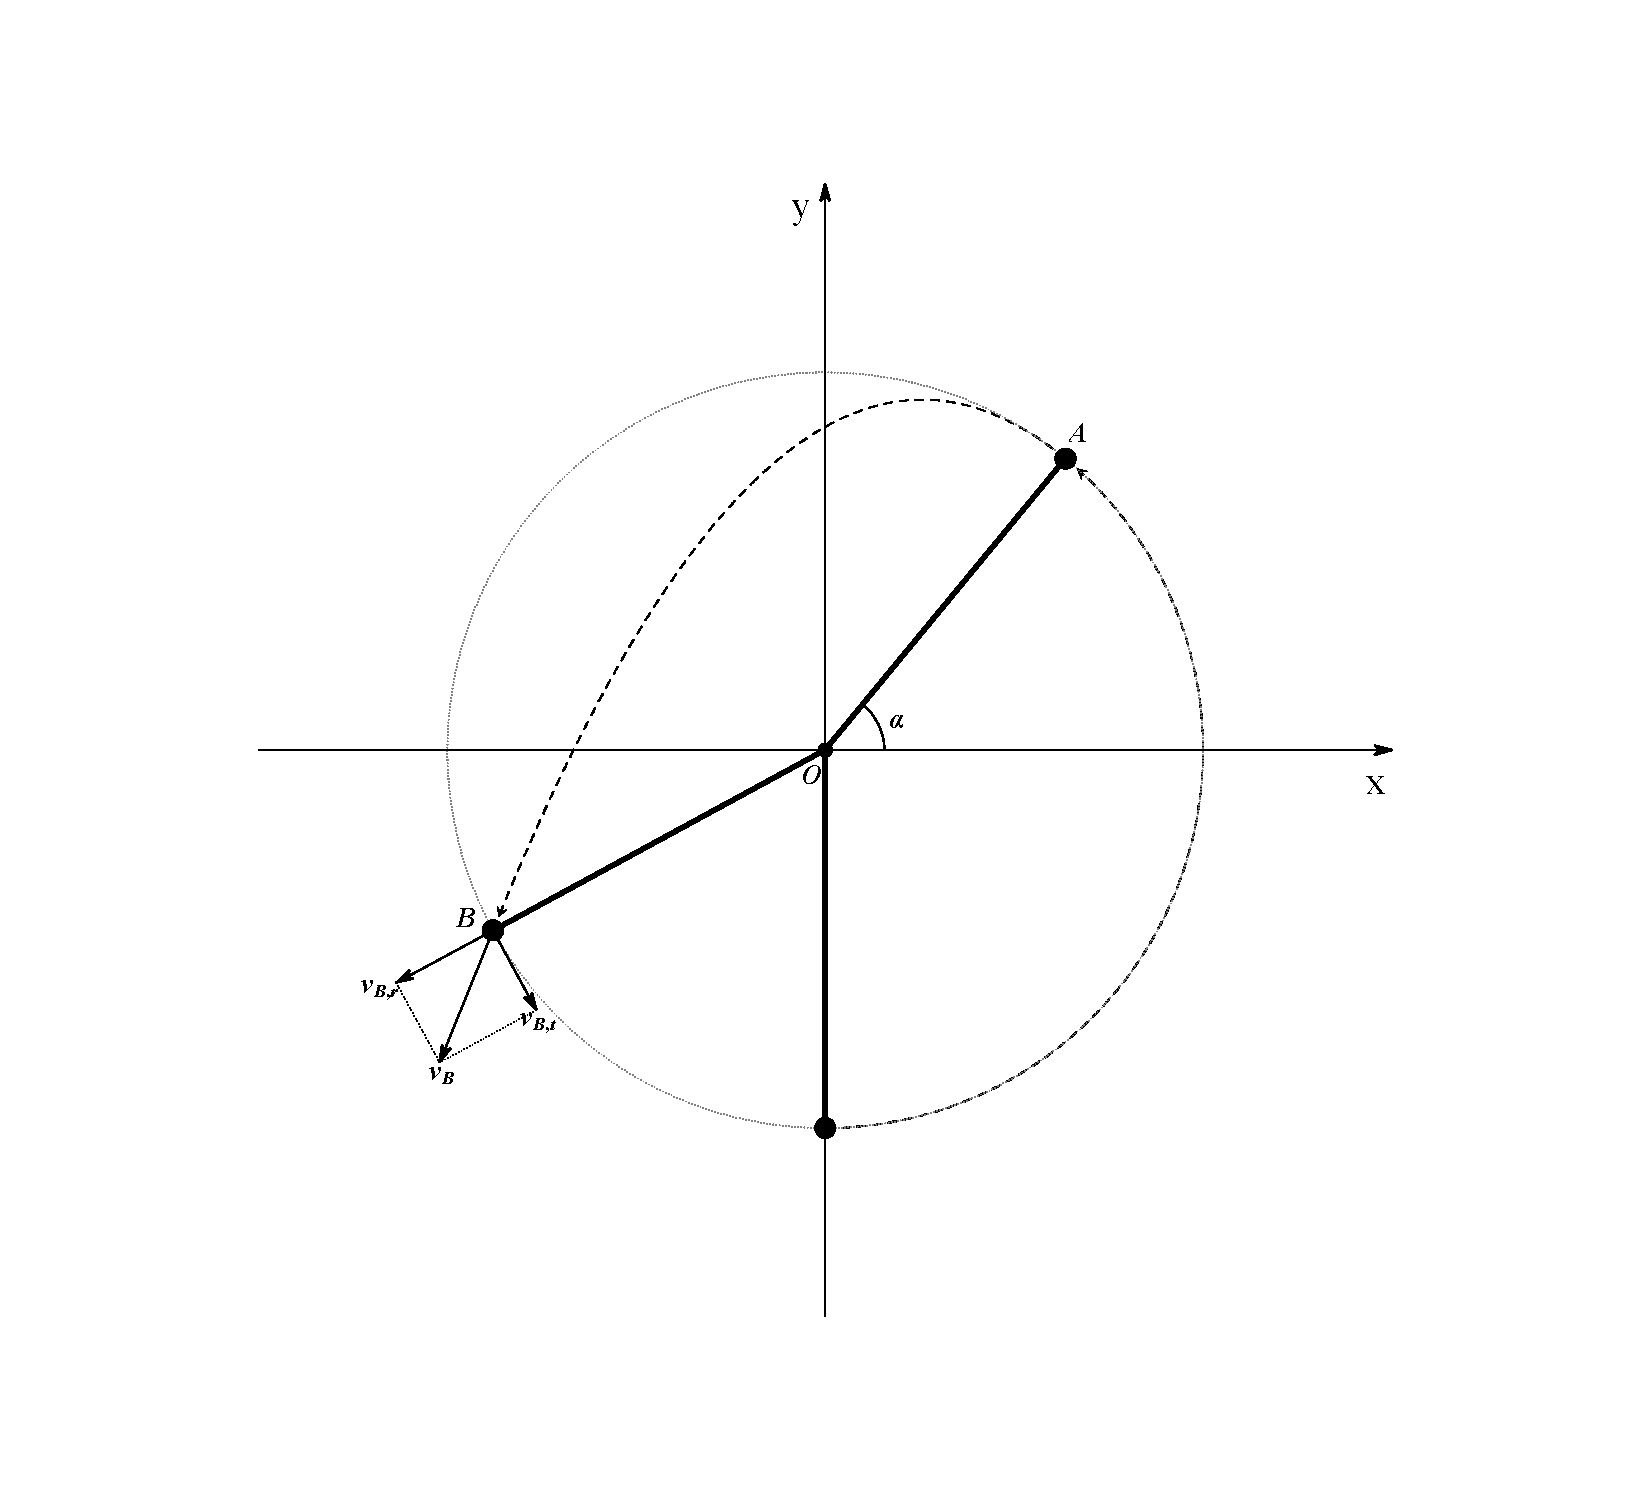
\includegraphics[scale=0.4]{system.pdf}
	\caption{System}
	\label{fig:sys}
\end{figure}

Assuming that the initial velocity of the ball is $v_0$ with the direction of x+. At the beginning, the ball travels along the circle and pass the horizontal point $(r, 0)$ and continue traveling up till a transition point before $(0, r)$. At the transition point, denoted as point $A$, the tension in the string decreases to zero, and the gravity starts to provide greater than the needed centripetal force, so after this point, the ball escapes from the circle path and starts projectile motion.

Denote the angle between $OA$ and x-axis as $\alpha \in (o, \pi/2)$, and the magnitude of velocity at point $A$ as $v_A$. On the one hand, the gravity provides the centripetal force at point A,
\[
mg\sin\alpha = \frac{mv_1^2}{r}  \quad\Rightarrow\quad gr\sin\alpha = v_1^2 \,;
\]
on the other hand, according to energy conservation,
\[
mgr(1+sin\alpha) + \frac{1}{2}mv_1^2 = 0 + E_0\,.
\]
Combining the two equation, we get
\begin{align*}
&&mgr(1+\sin\alpha) + \frac{1}{2}mgr\sin\alpha &= E_0 \\
\Rightarrow &&mgr(1 + \frac{3}{2}\sin\alpha) &= E_0 \\
\Rightarrow &&1 + \frac{3}{2}\sin\alpha &= \varepsilon_0 \\
\Rightarrow &&\sin\alpha &= \frac{2}{3}(\varepsilon_0 - 1)
\end{align*}

The ball travels along the parabola until it hits the circle path at point $B$. At this point, the string gains tension and cause energy loss. we need to calculate the coordinate and the velocity at point B in order to calculate the energy loss.

The ball starts the projectile motion at point $(r\cos\alpha, r\sin\alpha)$ with velocity $(-v_1\sin\alpha, v_1\cos\alpha)$, so the equations describing the motion in terms of time $t$ are
\begin{align*}
v_x &= -v_1\sin\alpha\,,\\
v_y &= v_1\cos\alpha - gt\,,\\
x &= r\cos\alpha-v_1t\sin\alpha\,,\\
y &= r\sin\alpha + v_1t\cos\alpha - \frac{1}{2}gt^2\,.
\end{align*}
Because point $B$ is on the circle, we have $x^2+y^2=r^2$. Substituting in the equation for $x$ and $y$, we get
\begin{align*}
&&(r\cos\alpha-v_1t\sin\alpha)^2 + (r\sin\alpha + v_1t\cos\alpha - \frac{1}{2}gt^2)^2 &= r^2\\
\Rightarrow && \uline{r^2\cos^2\alpha} -\uwave{2rv_1t\cos\alpha\sin\alpha} + \dashuline{v_1^2t^2\sin^2\alpha}\qquad& \\
&&+ \uline{r^2\sin^2\alpha} + \dashuline{v_1^2t^2\cos^2\alpha} + \frac{1}{4} g^2t^4\qquad& \\ &&+\uwave{2rv_1t\sin\alpha\cos\alpha} -\dashuline{grt^2\sin\alpha}-v_1gt^3\cos\alpha - \uline{r^2} &= 0\\
\Rightarrow && \dotuline{(v_1^2 - gr\sin\alpha)}t^2 -v_1gt^3\cos\alpha +  \frac{1}{4} g^2t^4 &= 0 \\
\Rightarrow && -v_1gt^3\cos\alpha +  \frac{1}{4} g^2t^4 &= 0 \\
\Rightarrow && t &= \frac{4v_1}{g}\cos\alpha\,.
\end{align*}
So the coordinates of point $B$ are
\begin{align*}
x_B &= r\cos\alpha-v_1t\sin\alpha \\
&=r\cos\alpha-\frac{4v_1^2}{g}\cos\alpha\sin\alpha\\
&=r\cos\alpha-4r\cos\alpha\sin^2\alpha\\
&=r\cos\alpha(1-4\sin^2\alpha)\\
&=r\cos3\alpha\,;\\
y_B &= r\sin\alpha + v_1t\cos\alpha - \frac{1}{2}gt^2\\
&=r\sin\alpha + \frac{4v_1^2}{g}\cos^2\alpha -\frac{8v_1^2}{g}\cos^2\alpha\\
&=r\sin\alpha - \frac{4v_1^2}{g}\cos^2\alpha\\
&=r\sin\alpha - 4r\sin\alpha\cos^2\alpha\\
&=r\sin\alpha(1-4\cos^2\alpha)\\
&=-r\sin3\alpha\,,
\end{align*}
and the velocity of the ball at point $B$ are
\begin{align*}
v_{B,x} & = -v_1\sin\alpha\,;\\
v_{B,y} & =v_1\cos\alpha - gt\\
&=v_1\cos\alpha - 4v_1\cos\alpha\\
&=-3v_1\cos\alpha\,.
\end{align*}
When the ball hits point $B$, its radial velocity vanishes. The radial velocity is
\begin{align*}
v_{B,r} &= \frac{\mathbf{r_B}\cdot\mathbf{v_B}}{\|\mathbf{r_B}\|}\\
&=\frac{x_Bv_{B,x}+y_Bv_{B,y}}{r}\\
&=\frac{-rv_1\cos3\alpha\sin\alpha+3rv_1\sin3\alpha\cos\alpha}{r}\\
&=v_1(-\cos3\alpha\sin\alpha+3\sin3\alpha\cos\alpha)\\
&=8v_1\sin\alpha\cos^3\alpha\,.
\end{align*}
So the energy loss at point $B$ is
\begin{align*}
\Delta E_B &= \frac{1}{2}mv_{B,r}^2\\
&=\frac{1}{2}m\cdot64v_1^2\sin^2\alpha\cos^6\alpha\\
&=\frac{1}{2}m\cdot64gr\sin^3\alpha\cos^6\alpha\\
&=32mgr\sin^3\alpha\cos^6\alpha\,,\\
\end{align*}
which, expressed in terms of dimensionless energy, is
\begin{align*}
\Delta \varepsilon_B &= 32\sin^3\alpha\cos^6\alpha \\
&=32 \sin^3\alpha (1-\sin^2\alpha)^3 \\
&=32 \Big(\frac{2}{3}(\varepsilon_0 -1)\Big)^3 \Big(1-\Big(\frac{2}{3}(\varepsilon_0 -1)\Big)^2\Big)^3\,.
\end{align*}
So the mechanical energy of the ball after point B is
\begin{align*}
\varepsilon_1 &= \varepsilon_0 - \Delta \varepsilon_B\\
 &= \varepsilon_0 -32 \Big(\frac{2}{3}(\varepsilon_0 -1)\Big)^3 \Big(1-\Big(\frac{2}{3}(\varepsilon_0 -1)\Big)^2\Big)^3\,.
\end{align*}	
We also need to consider whether the ball travels along the circle path or goes in another projectile motion after point $B$. To do this, we compare the tangential velocity and the centripetal force provided by gravity. The tangential velocity is
\begin{align*}
v_{B,t} &= \frac{\mathbf{r_B}\times\mathbf{v_B}}{\|\mathbf{r_B}\|}\\
&= \frac{x_Bv_{B,y}-y_Bv_{B,x}}{r}\\
&= \frac{-3rv_1\cos3\alpha\cos\alpha-rv_1\sin3\alpha\sin\alpha}{r} \\ 
&= -v_1(3\cos3\alpha\cos\alpha + \sin3\alpha\sin\alpha)\,.
\end{align*}
And the gravity force on the radial direction (outward as positive) is
\begin{align*}
G_t &= \frac{\mathbf{r_B}\cdot\mathbf{G}}{\|\mathbf{r_B}\|}\\
 &=\frac{mgr\sin3\alpha}{r}\\
 &=mg\sin3\alpha\,,
\end{align*}
so the force equilibrium at point $B$ is
\begin{align*}
&&T - G_t &= \frac{mv_{B,t}^2}{r}  \\
\Rightarrow &&T - mg\sin3\alpha &= \frac{mv_1^2}{r}(3\cos3\alpha\cos\alpha + \sin3\alpha\sin\alpha)^2 \\
\Rightarrow &&T &= mg(\sin\alpha(3\cos3\alpha\cos\alpha + \sin3\alpha\sin\alpha)^2+\sin3\alpha)\,.
\end{align*}
It can be proven that the RHS is always positive for $\alpha\in(0,\pi/2)$ (See Section \ref{sec:RHS-positive} for detail), so the circular motion at points $B$ always require tension in the string, which means the ball is kept on the circle path. From this point, it is equivalent to a system where the ball has an initial kinetic energy $\varepsilon_1$. If this energy is below 1, the system becomes a pendulum; otherwise in the next time the ball will escapes from the circle path, travels in parabola, hits the circle path again and lose more energy to $\varepsilon_2$, and so on. The energy of the $n$-th stage is a function of previous stage
\[
\varepsilon_n = f(\varepsilon_{n-1})\,,
\]
and the function, as previously analyzed, is
\[
f(\varepsilon) = \left\{ \begin{array}{ll}
\varepsilon & \textrm{if $\varepsilon \in [0, 1]$ or $\varepsilon \in [2.5, \infty)$} \\
\varepsilon -32 \Big(\frac{2}{3}(\varepsilon -1)\Big)^3 \Big(1-\Big(\frac{2}{3}(\varepsilon -1)\Big)^2\Big)^3 & \textrm{if $\varepsilon \in (1, 2.5)$}
\end{array}\right.
\]
The final energy $\varepsilon_\infty$ is simply the infinite recursion of this function
\[
\varepsilon_\infty=\lim\limits_{n\rightarrow\infty}\varepsilon_n = f(f(...f(\varepsilon_0))) = F(\varepsilon_0) \,.
\]

\section{The Graph}

In this section we study the properties of the function $f(\varepsilon)$ and its recursive version $F(\varepsilon)$.

\subsection{One Iteration}

The graph of function $f(\varepsilon)$ is shown in Figure \ref{fig:f1}. The interesting part is between $\varepsilon_0 = 1$ and $\varepsilon_0=2.5$, where there is energy loss. There are two critical points that split this range into three region: $\varepsilon_0 \approx 1.35$ and $\varepsilon_0 \approx 2.13$.

\begin{figure}[!h]
	\centering
	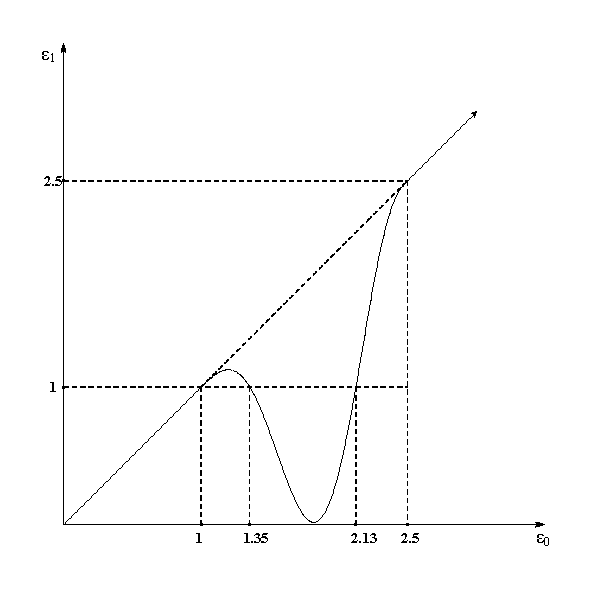
\includegraphics[scale=1]{f1.pdf}
	\caption{Function $f(\varepsilon)$}
	\label{fig:f1}
\end{figure}

In the first region, the total energy after the energy loss is still above 1, so it will have another energy loss in the next turn. 

In the second region, the total energy is below 1, and the ball will travel as pendulum and there is no more energy loss. It is worth to note that the minimum point in this region, although very close, is not exactly zero. A zero total energy requires that (1) the parabola path intersects the circle path at the lowest point where potential energy is zero, and (2) the two path are perpendicular to each other at the intersection to cancel all velocity the ball has to reach zero kinetic energy. These two requirements cannot be achieved at the same time. The first requirement is achieved at $\varepsilon_0 = 1.75$ and the second one is at $\varepsilon_0 = 1+3\sqrt{3-\sqrt{3}}/4 \approx 1.84$ (see Section \ref{sec:perp} for detail). The minimum point is at $\varepsilon_0 \approx 1.82, \varepsilon_1 \approx 0.018$, just between the two points.

In the third region, the total energy is above 1 again, and more energy loss will happen in the next turn.

\subsection{Two Iteration}

Now let's apply recursion to the function, and study the graph of $f(f(\varepsilon))$. Only in range $\varepsilon \in (1, 1.35)$ and $\varepsilon \in (2.13, 2.5)$ the ball will lose energy in the second tern, and the graph shape will change. 

\begin{figure}[!h]
	\centering
	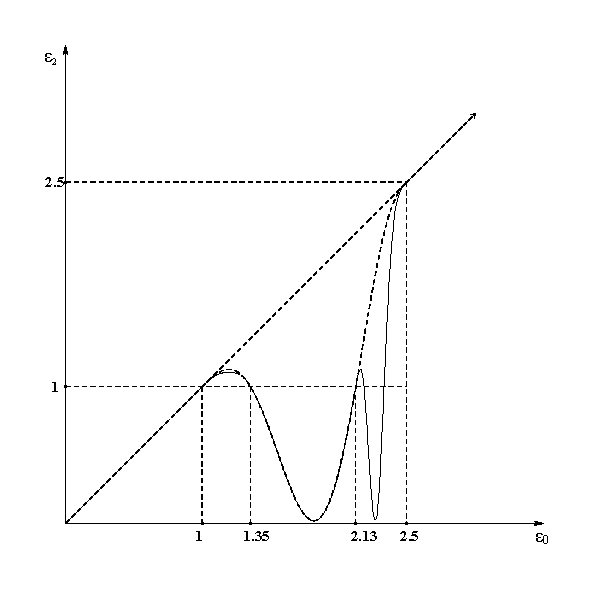
\includegraphics[scale=1]{f2.pdf}
	\caption{Function $f(f(\varepsilon))$}
	\label{fig:f2}
\end{figure}

In the range $\varepsilon \in (1, 1.35)$, the range of image $f(\varepsilon)$ is a subset of the preimage $\varepsilon$, so the recursion will only "contract" this subset more, resulting a flatter curve.

In the range  $\varepsilon \in (2.3, 2.5)$, the range of image $f(\varepsilon)$ goes through the entire range $(1, 2.5)$, resulting a "clone" of the function from $(1, 2.5)$ to $(2.13, 2.5)$

\subsection{Infinite Iteration}

After infinite recursion, values in $(1, 1.35)$ converge to the fixed point $\varepsilon_\infty = 1$, while values $(2.3, 2.5)$ continues map range $(1, 2.5)$ onto itself, forming a self-similar infinite oscillation between 0 and 1.
The function has an essential discontinuity at $\varepsilon_0 = 2.5$, and continuous at any other points.
\begin{figure}[!h]
	\centering
	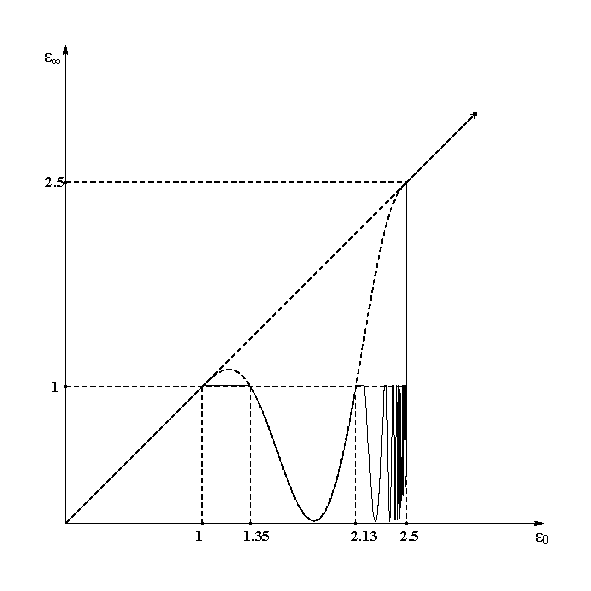
\includegraphics[scale=1]{fb.pdf}
	\caption{Function $F(\varepsilon)$}
	\label{fig:fb}
\end{figure}

\section{The Extra}

\subsection{When the parabola intersects the circle at the lowest point}
\label{sec:low}
This means the y-coordinate of B is $-r$, which is
\begin{align*}
&&-r\sin3\alpha&=-r\\
\Rightarrow &&\sin3\alpha &= 1\\
\Rightarrow &&\alpha &= \frac{\pi}{6}\\
\Rightarrow &&\varepsilon_0 = 1+\frac{3}{2}\sin\alpha&=\frac{7}{4}\,.
\end{align*}

\subsection{When the parabola is perpendicular to the circle}
\label{sec:perp}
This means the tangential velocity of the ball at the intersection is zero, which means
\begin{align*}
&&3\cos3\alpha\cos\alpha+\sin3\alpha\sin\alpha&=0 \\
\Rightarrow && \frac{3}{2}\cos2\alpha+\frac{3}{2}\cos4\alpha+\frac{1}{2}\cos2\alpha-\frac{1}{2}\cos4\alpha &= 0\\
\Rightarrow &&2\cos2\alpha+\cos4\alpha &= 0 \\
\Rightarrow &&2\cos2\alpha+2\cos^22\alpha-1 &=0\\
\Rightarrow &&\cos2\alpha &= -\frac{1}{2}\pm\frac{\sqrt{3}}{2}\\
\Rightarrow &&1-2\sin^2\alpha &= -\frac{1}{2}\pm\frac{\sqrt{3}}{2} \\
\Rightarrow &&\sin\alpha &= \frac{\sqrt{3-\sqrt{3}}}{2}\\
\Rightarrow &&\varepsilon_0 = 1+\frac{3}{2}\sin\alpha&=1+\frac{3\sqrt{3-\sqrt{3}}}{4}\,.
\end{align*}

\subsection{The positivity of a trigonometric expression}
\label{sec:RHS-positive}

The expression can be rearranged as
\begin{align*}
&\sin\alpha(3\cos3\alpha\cos\alpha + \sin3\alpha\sin\alpha)^2+\sin3\alpha \\
=&\sin\alpha(3\cos3\alpha\cos\alpha + \sin3\alpha\sin\alpha)^2 + 3\sin\alpha-4\sin\alpha\sin^3\alpha \\
=&\sin\alpha((3\cos3\alpha\cos\alpha + \sin3\alpha\sin\alpha)^2 + 3-4\sin^3\alpha) \\
=&\sin\alpha((\frac{3}{2}\cos2\alpha+\frac{3}{2}\cos4\alpha+\frac{1}{2}\cos2\alpha-\frac{1}{2}\cos4\alpha)^2 + 4\cos^2\alpha-1)\\
=&\sin\alpha((2\cos2\alpha+\cos4\alpha)^2 + 4\cos^2\alpha-1)\\
=&\sin\alpha((2\cos2\alpha+2\cos^22\alpha-1)^2 + 2\cos2\alpha+1)\,.
\end{align*}
For $\alpha\in(0, \pi/2)$, we have $\sin\alpha\in(0, 1)$ and $\cos2\alpha\in(-1, 1)$. To prove that the expression is positive, we only need to prove the positivity of polynomial $(2x^2+2x-1)^2+2x+1$ for $x \in (-1,1)$. The polynomial can be rearranged as
\begin{align*}
&(2x^2+2x-1)^2+2x+1\\
=&4x^4+8x^3-2x+2\\
=&(x-1)(2x^3+2x^2-2x+1)\,.
\end{align*}
Since $x-1>0$, we only need to prove $g(x) = 2x^3+2x^2-2x+1 > 0$. For this cubic function, we consider its derivative
\begin{align*}
g'(x)=&(2x^3+2x^2-2x+1)'\\
=&6x^2+4x-2\\
=&(x+1)(6x-2)\,,
\end{align*}
and we using the derivative we can summarize the monotonicity and local extrema of $g(x)$ in Table \ref{tab:g}.
\begin{table}[!h]
	\centering
	\caption{Monotonicity and local extrema of $g(x) = 2x^3+2x^2-2x+1$}
	\begin{tabular}{c|ccccc}
		\hline
		$x$&$(-\infty,-1)$&$-1$&$(-1, 1/3)$&$1/3$&$(1/3, +\infty)$\\
		\hline
		$g'(x)$&$+$&$0$&$-$&$0$&$+$\\
		\hline
		$g(x)$&$\nearrow$&$3$ (max)&$\searrow$&$17/27$ (min)&$\nearrow$\\
		\hline
	\end{tabular}
\label{tab:g}
\end{table}
So the minimum point of $g(x)$ in $x\in(-1,1)$ is $g(1/3) = 17/27 > 0$, and there for $g(x) > 0$ for $x\in(-1,1)$.



\end{document}